
Las ondas sonoras son oscilaciones longitudinales que provocan variaciones en la presión del medio, como por ejemplo, un pistón generando ruido al final de un tubo al moverse a través de el en la Figura \ref{fig:ondas}, zonas más densas (compresiones) y zonas menos densas (rarefacciones). Se generan por una fuente vibratoria, como una cuerda, un altavoz, cuerdas vocales o una gota de agua y esa vibración se transmite por colisión entre partículas del medio. \cite{sbe_sound}

\begin{figure}[H]
    \centering
    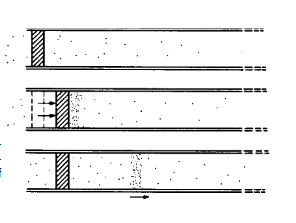
\includegraphics[width=0.7\textwidth]{commons/Fig1.png}
    \caption{Generación de una onda sonora longitudinal mediante el movimiento de un pistón al final de un tubo \cite{sbe_sound}.}
    \label{fig:ondas}
\end{figure}
